\subsection{Modèle existant} 
Dans cette section, la première approche pour détecter le type de traverse contenu dans un segment est examinée. Cette méthode, déjà existante, repose sur une approche mathématique qui est assez performante, mais qui est sujette à des limitations dans des conditions spécifiques (\textit{cf.} Section 5.2.1). L'identification de la traverse se base sur les profils qui se trouvent dans la Zone 2 (\textit{cf.} Section 2.2). \\

\noindent Cette approche, développée en Java, est décomposée en 3 étapes. Dans la première étape (cf. Section 5.1.1), les profils présents dans un segment sont filtrés pour ne garder que ceux contenant des traverses. Ensuite (\textit{cf.} Section 5.1.2), ces profils sont analysés pour identifier le type spécifique de traverse. Enfin (\textit{cf.} Section 5.1.3), un tableau recense toutes les traverses identifiées avec leur fréquence d'apparition, ce tableau étant utilisé comme score pour déterminer le type du segment.


\subsubsection{Tri des profils}


L'analyse du type de traverse débute par un filtrage des profils contenus dans un segment afin de ne conserver que ceux qui contiennent des traverses. Pour ce faire, on se base sur deux zones plates qui sont communes à toutes les traverses, comme illustré par la Figure 14.  

\begin{figure}[H]
            \centering

           \fbox{ 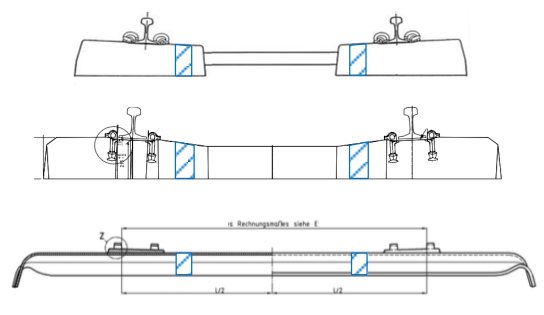
\includegraphics[width=7.5cm]{images/sleepers_flat.png}}   
            \caption{Partie plate commune à toutes les traverses - Cegelec \cite{RHEA}} 
        \end{figure}

\noindent Ensuite, des fonctions polynomiales du premier degré sont appliquées sur ces zones afin de comparer l'écart-type de la régression avec un seuil prédéfini de 2,5. Si l'écart-type dans l'une des deux zones est inférieur à ce seuil, le profil est considéré comme celui d'une traverse (\textit{cf.} Figure 15a) ; sinon, il est classé comme étant du ballast (\textit{cf.} Figure 15b).
 
 \begin{figure}[H]
      \centering
      \fbox{\subcaptionbox{Profil contenant une traverse}{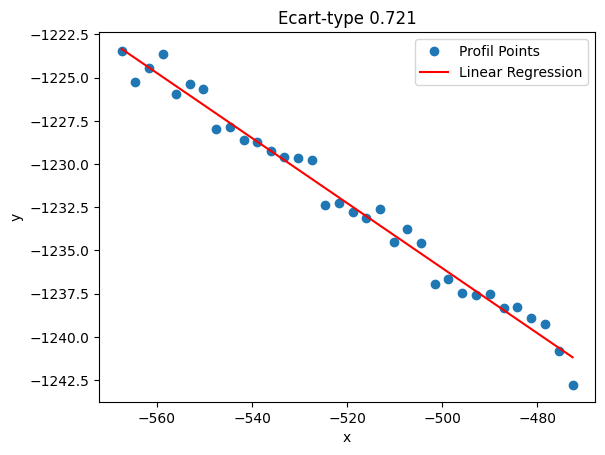
\includegraphics[width=6cm]{images/sleepers_detection_yes.png}}}
      \qquad % Add some space between the two subfigures
      \fbox{\subcaptionbox{Profil contenant du ballast}{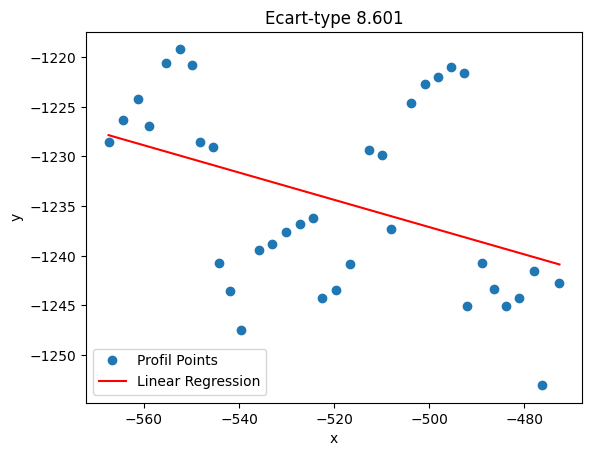
\includegraphics[width=5.8cm]{images/sleepers_detection_no.png}}}

      \caption{Identification du profil contenant une traverse versus ballast}

    \end{figure}
        

\subsubsection{Identification du type de traverse}
Pour identifier le type de traverse, une méthode statique est utilisée, s'appuyant sur une bibliothèque de profils de référence disponibles dans un fichier JSON. Ces profils théoriques sont dérivés des plans compilés et définissent la forme à suivre pour chaque type de traverse. \\

\noindent Le processus d'identification se déroule en plusieurs étapes.
\begin{itemize}
\item Tout d'abord, une hauteur de référence est déterminée en fonction de la configuration spécifique de la traverse. Les emplacements dans la zone x, définis dans la bibliothèque, indiquent où mesurer cette hauteur de référence. Le choix stratégique de la zone x vise à générer des écarts en fonction du type de traverse.

\item Par la suite, le profil mesuré et le profil théorique sont comparés en les superposant sur leurs points de hauteur de référence, et l'écart entre les deux est déterminé. Ce dernier est quantifié en calculant l'intégrale des différences entre les deux profils (\textit{cf.} Figure 16).

\item Enfin, un score est calculé pour chaque type de traverse en fonction de la surface d'écart obtenue lors de la comparaison. Un score plus faible indique une meilleure correspondance entre le profil mesuré et le modèle théorique.

\end{itemize}
\begin{figure}[H]
            \centering

           \fbox{ 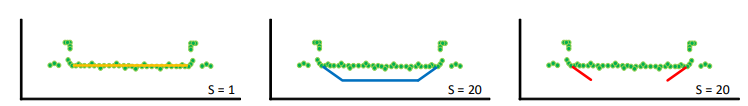
\includegraphics[width=12cm]{images/identification_sleepers.png}}   
            \caption{Identification de la traverse - Cegelec \cite{RHEA}} 
        \end{figure}


\subsubsection{Identification du type de segment}
L'identification du type de segment repose sur l'analyse d'un tableau qui répertorie, pour chaque type de traverse, le nombre de profils qui lui sont associés ainsi que la moyenne des scores de correspondance de ces profils (\textit{cf.} Figure 17). Le type de traverse attribué au segment est celui dont les profils associés ont le meilleur score. \\

\begin{figure}[H]
            \centering

           \fbox{ 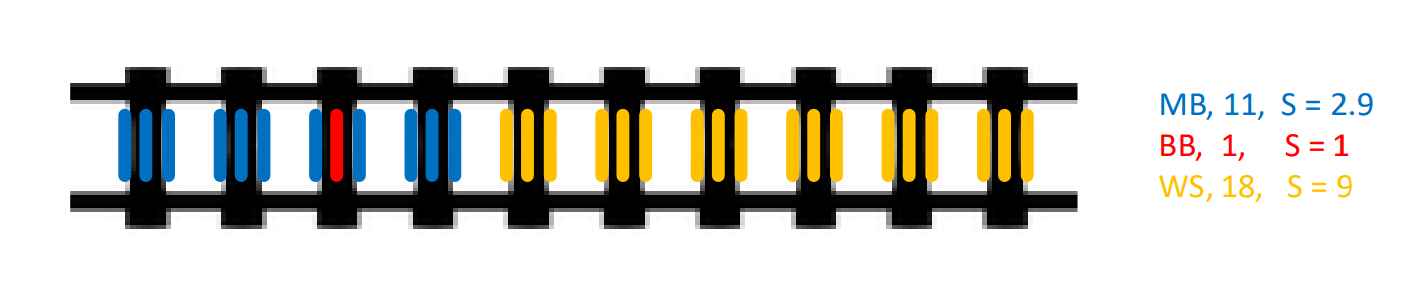
\includegraphics[width=10cm]{images/segment_identification.png}}   
            \caption{Identification du type de segment - Cegelec \cite{RHEA}} 
        \end{figure}

\noindent Cependant, des règles de vote sont appliquées lors de l'analyse des profils de segments. Si tous les profils sont jugés de mauvaise qualité, le segment est rejeté. De même, si la majorité des profils ont un score de correspondance supérieur à 20, le segment est également rejeté. Ces règles garantissent la fiabilité de l'identification du type de segment.


\subsubsection{Limites du modèle}
% % Discutez des limites ou des lacunes du modèle mathématique existant.
% % Identifiez les aspects pour lesquels l'intelligence artificielle peut apporter des améliorations.Actuellement, la première approche développée en Java pour détecter le type de traverse repose sur une méthode mathématique qui fonctionne de manière raisonnable. Toutefois, certaines limitations se manifestent dans des conditions spécifiques, telles qu'une quantité accrue de ballast, la présence de rouille sur les traverses, des buissons ou une végétation \\

% En résumé, cette méthode d'identification du type de traverse dans un segment propose une approche bien structurée en trois étapes distinctes. D'abord, elle effectue un filtrage des profils pour ne conserver que ceux qui contiennent des traverses, puis elle procède à une analyse approfondie pour déterminer le type spécifique de traverse. Enfin, elle se sert d'un tableau répertoriant les types de traverses identifiés avec leurs fréquences d'apparition et leurs scores pour conclure sur le type du segment.\\

% \noindent Cependant, 
Bien que cette méthode soit performante dans de nombreuses situations, elle présente des lacunes dans des conditions où des facteurs perturbateurs tels que la végétation ou la rouille peuvent affecter la précision de la détection. De plus, certains types de traverses moins courants sur le terrain, ainsi que les segments contenant des composants spécifiques tels que des crocodiles ou des balises ETCS, ne sont pas pris en compte dans le processus d'identification. \\

\noindent Malgré ces limitations, cette méthode reste efficace dans de nombreuses situations. Néanmoins, les variations subtiles peuvent représenter des défis significatifs, mettant en évidence la nécessité d'explorer des approches alternatives. Par exemple, l'utilisation de techniques basées sur l'intelligence artificielle pourrait offrir des solutions plus robustes et adaptatives.

